% Generated atomically by embed-optim-render-paper-results.
\begin{figure*}[t]
\centering
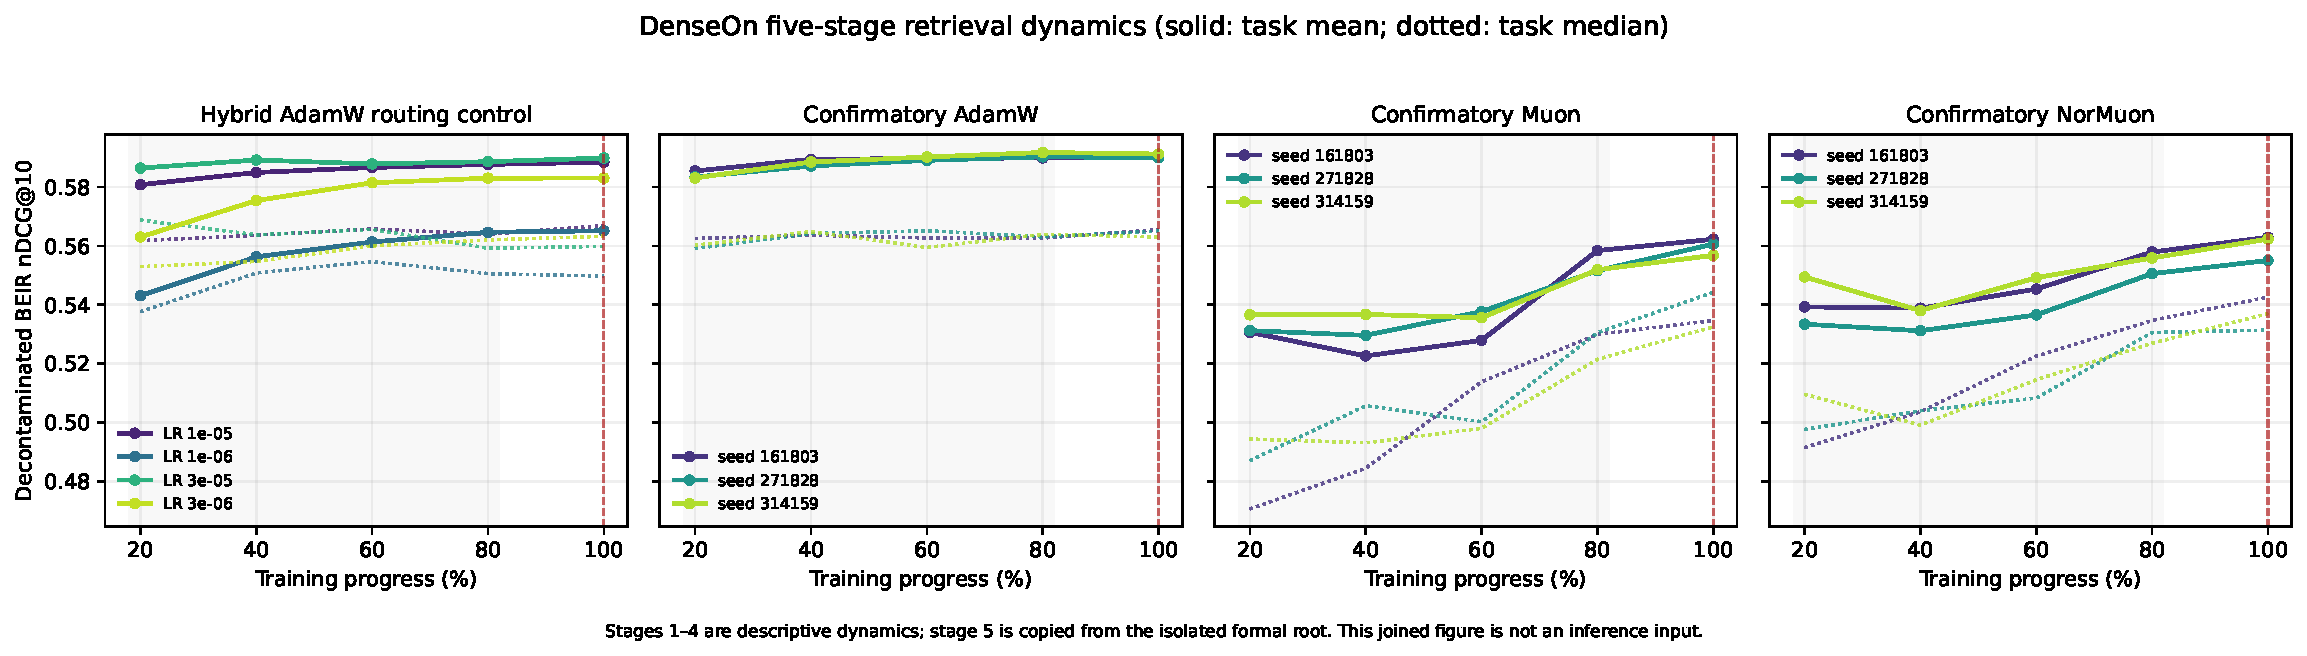
\includegraphics[width=\textwidth]{../reports/dense-retrieval-dynamics/five_stage_retrieval_dynamics.pdf}
\caption{Descriptive five-stage decontaminated-BEIR trajectories for the four routing-matched hybrid runs and nine validation-frozen confirmatory runs. Stages 1--4 come from isolated dynamics roots; stage 5 is joined from the pre-existing formal roots. This figure is not an inference input.}
\label{fig:extended-retrieval-dynamics}
\end{figure*}

\begin{table*}[t]
\centering
\small
\begin{tabular}{lrrrrrr}
\toprule
Series & Runs & 20\% & 40\% & 60\% & 80\% & 100\% \\
\midrule
Hybrid AdamW & 4 & 0.5684 & 0.5765 & 0.5794 & 0.5810 & 0.5817 \\
Confirmatory AdamW & 3 & 0.5840 & 0.5884 & 0.5897 & 0.5907 & 0.5905 \\
Confirmatory Muon & 3 & 0.5328 & 0.5296 & 0.5337 & 0.5540 & 0.5599 \\
Confirmatory NorMuon & 3 & 0.5407 & 0.5360 & 0.5437 & 0.5548 & 0.5601 \\
\bottomrule
\end{tabular}
\caption{Mean nDCG@10 across the four hybrid learning-rate runs or three new seeds per optimizer. These are descriptive aggregates of the source-bound 65-row CSV, not additional formal contrasts.}
\label{tab:extended-retrieval-dynamics}
\end{table*}

\paragraph{Descriptive time-to-quality.} Using mean stage-5 confirmatory AdamW nDCG@10 (0.5905) as the displayed four-decimal fixed reference, the earliest retained checkpoint matching or exceeding it is: AdamW 80\%; Muon not reached; NorMuon not reached. Normalized 20--100\% trajectory AUC is: AdamW 0.5890, Muon 0.5409, NorMuon 0.5462. Checkpoint attainment and AUC summarize the joined curves only; they do not alter the stage-5 confirmatory test.
